\documentclass[a4paper, 12pt]{article}
\usepackage[UTF8]{ctex}
\usepackage{geometry}
\usepackage{graphicx}
\usepackage{array}
\usepackage{xcolor}
\usepackage{listings}
\usepackage{enumitem}
\usepackage{hyperref}
\usepackage{amsmath}
\usepackage{tikz}
\usepackage{float}     % 提供 [H] 浮动控制符
\usetikzlibrary{arrows, positioning}

% 列表设置
\setlist[itemize]{leftmargin=*, nosep}
\setlist[enumerate]{leftmargin=*, nosep}

\title{数据库系统实验课程设计报告}
\author{
    郑皓 \\ 姚书璟\\ 罗斯
    \and
    学号：23336328  \\ 学号：23336386 \\ 学号：xxx
    \and
    班级：9 \\ 班级：8 \\ 班级：9
}
\date{提交时间：\rule{3cm}{0.4pt} 年 \rule{2cm}{0.4pt} 月 \rule{2cm}{0.4pt} 日}

% ========== 解决中文代码注释问题 ==========
\usepackage{listings}
\usepackage{xeCJK}
\setCJKmainfont{SimSun}
% 代码块设置
\lstset{
    basicstyle=\ttfamily\small,
    breaklines=true,
    extendedchars=true,
    keepspaces=true,
    commentstyle=\color{gray}\itshape,
    escapeinside=``,
    numbers=left,
    numberstyle=\tiny\color{gray},
    frame=single,
    tabsize=4
}

\begin{document}
\maketitle

\section*{题目}
以miniob为基础的数据库设计

\section{开发环境与开发工具}
\begin{itemize}
    \item Docker, Visual Studio Code
    \item MiniOB: OceanBase团队基于华中科技大学数据库课程原型开发的入门学习项目
\end{itemize}

\subsection*{MiniOB 架构}
\begin{center}
    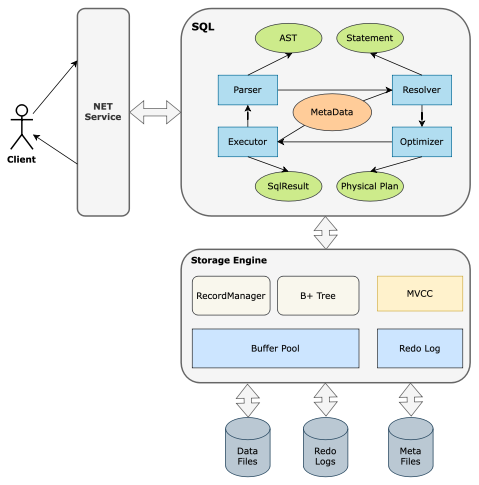
\includegraphics[width=0.8\textwidth]{miniob_arch.png}
\end{center}

\begin{itemize}
    \item 网络模块(NET Service)：负责与客户端交互
    \item SQL解析(Parser)：将SQL语句解析成语法树
    \item 语义解析(Resolver)：语法树转内部数据结构
    \item 查询优化(Optimizer)：调整/重写语法树
    \item 计划执行(Executor)：执行并生成结果
    \item 存储引擎(Storage Engine)：数据存储和检索
    \item 事务管理(MVCC)：管理事务提交、回滚
    \item 日志管理(Redo Log)：记录操作日志
    \item B+ Tree：索引存储结构
\end{itemize}

\subsection*{\heiti 表文件管理}
\begin{figure}[H]
  \centering
  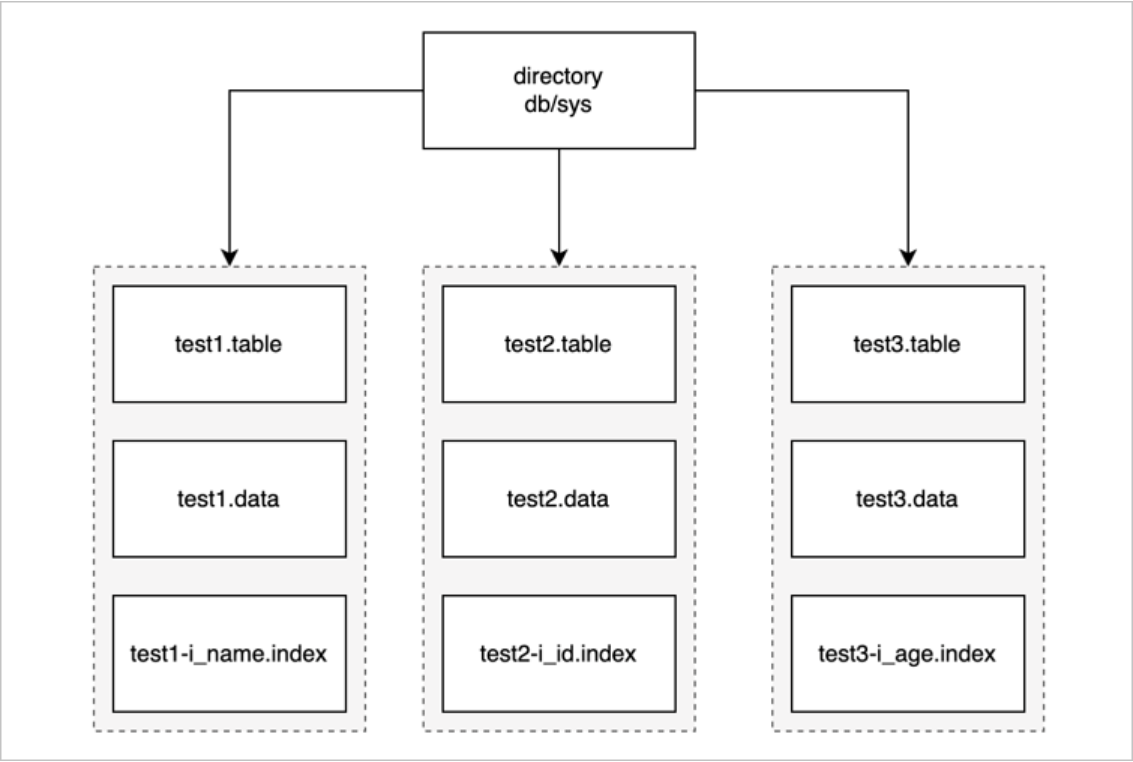
\includegraphics[width=0.6\textwidth]{file-arange.png}
  \caption{表文件组织方式图}
\end{figure}

\begin{itemize}
    \item test1.table：元数据文件，这里面存放了一些元数据。如：表名、数据的索引、字段类型、类型长度等。
    \item test1.data：数据文件，真正记录存放的文件。
    \item test1-i\_name.index：索引文件，索引文件有很多个，这里只展示一个示例。
\end{itemize}


\subsection*{\heiti 缓冲区结构}
\begin{figure}[H]
  \centering
  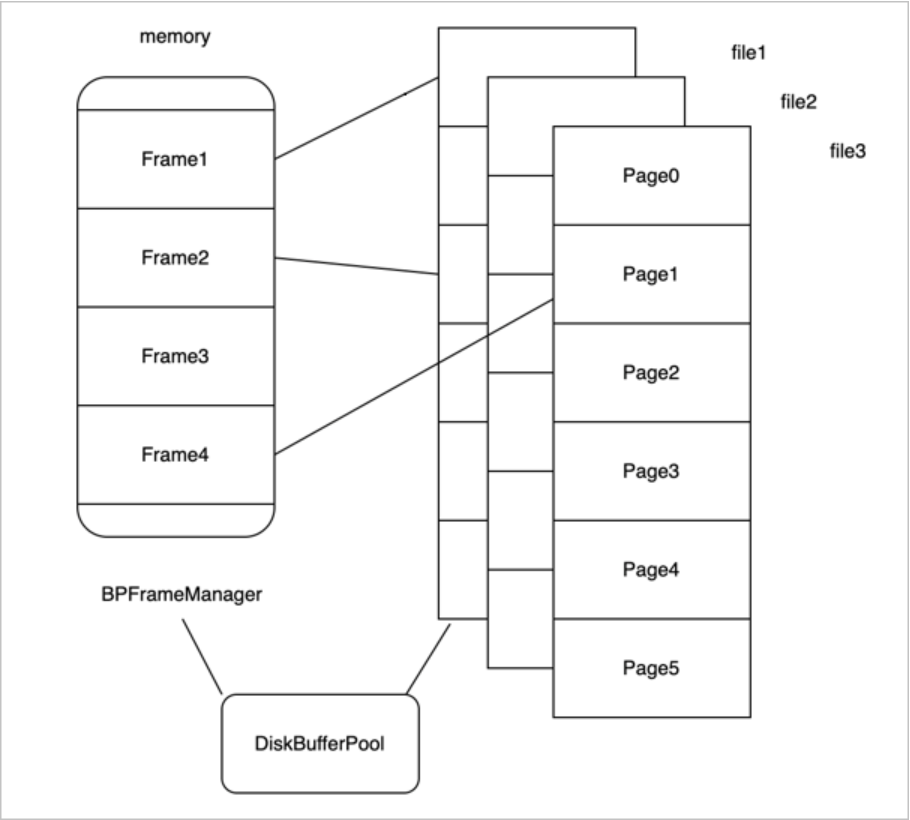
\includegraphics[width=0.6\textwidth]{buffer-pool.png}
  \caption{缓冲区结构示意图}
\end{figure}

\paragraph{\heiti 概述}

MiniOB 的缓冲区采用典型的 Buffer Pool 机制。内存被划分为若干固定大小的页帧（frame），磁盘文件按固定大小的页（page）组织，每个 page 在内存中至多对应一个 frame，二者大小一致，数据交换以页为单位进行。

在实现上，每个物理文件对应一个 DiskBufferPool 对象，而所有 DiskBufferPool 共享统一的页帧管理组件 BPFrameManager，由其负责 frame 的分配、回收与淘汰。

当访问某个磁盘页面时，系统首先在 BPFrameManager 中查找空闲 frame；若存在，则将该 frame 与目标 page 绑定，并将页面数据读入内存。若内存中不存在空闲 frame，则需要从已占用的 frame 中选择一个进行淘汰，将其解除绑定后，重新关联到新页面并加载数据。

MiniOB 采用 LRU（Least Recently Used）算法 作为页面替换策略，以优先淘汰最近最少使用的页面。

\subsection*{\heiti 文件结构}
\begin{figure}[H]
  \centering
  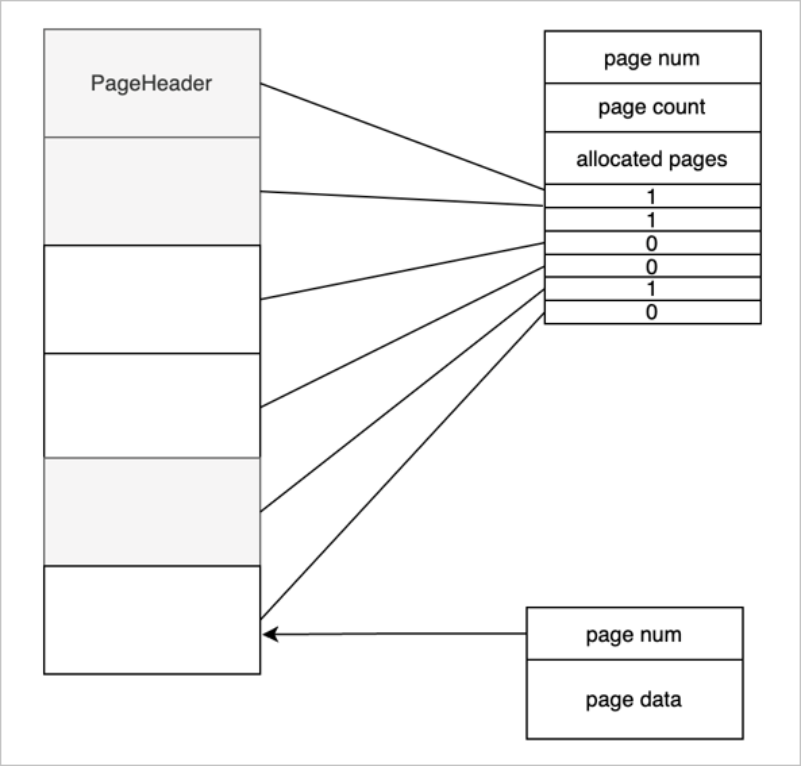
\includegraphics[width=0.6\textwidth]{file-structure.png}
  \caption{文件结构图}
\end{figure}

\begin{itemize}
    \item 文件上的第一页称为页头或文件头。文件头是一个特殊的页面，这个页面上会存放一个页号，这个页号肯定都是零号页，即 page num 是 0。
    \item page count 表示当前的文件一共有多少个页面。
    \item allocated pages 表示已经分配了多少个页面。如图所示标灰的是已经分配的三个页面。
    \item Bitmap 表示每一个 bit 位当前对应的页面的分配状态，1 已分配页面，0 空闲页面。
\end{itemize}


\subsection*{\heiti 记录管理}
\begin{figure}[H]
  \centering
  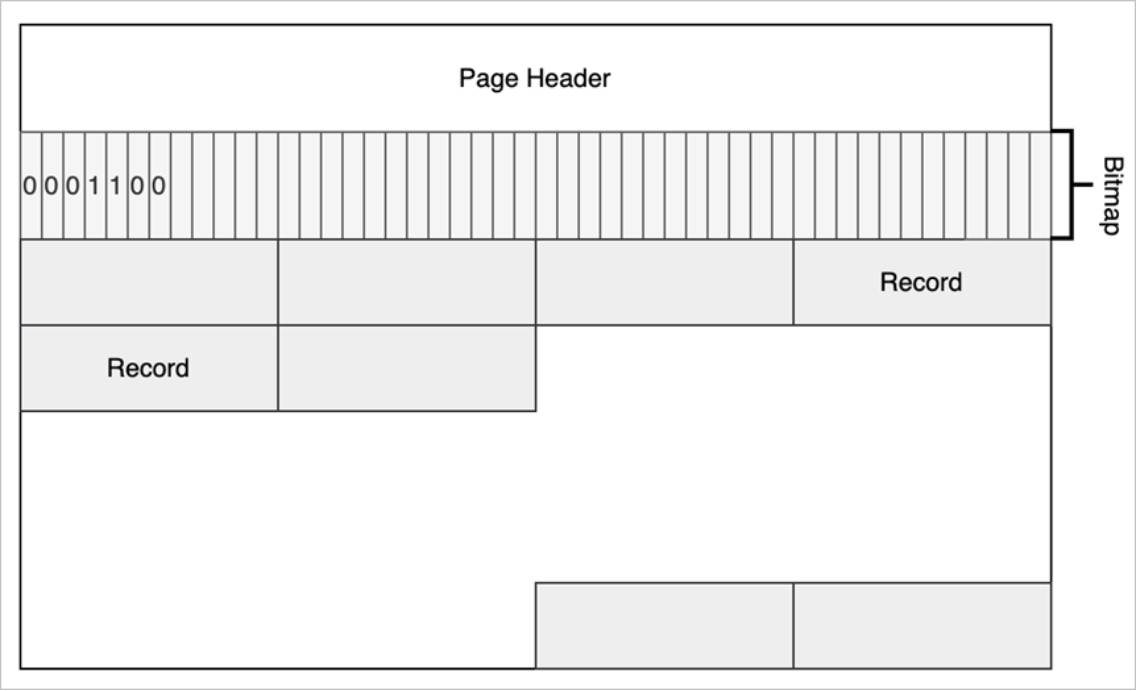
\includegraphics[width=0.6\textwidth]{record-manage.png}
  \caption{记录管理结构图}
\end{figure}

\paragraph{\heiti 简述}

Record Manager 是在 Buffer Pool 的基础上实现的，比如 page0 是 Buffer Pool 里面使用的元数据，Record Manager 利用了其他的一些页面。每个页面有一个头信息 Page Header，一个 Bitmap，Bitmap 为 0 表示最近的记录是不是已经有有效数据；1 表示有有效数据。Page Header 中记录了当前页面一共有多少记录、最多可以容纳多少记录、每个记录的实际长度与对齐后的长度等信息。

\subsection*{\heiti B+树}

\paragraph{索引文件}
每一个索引文件都存储着一棵B+树，其第一个page为树的根节点。

\begin{figure}[H]
  \centering
  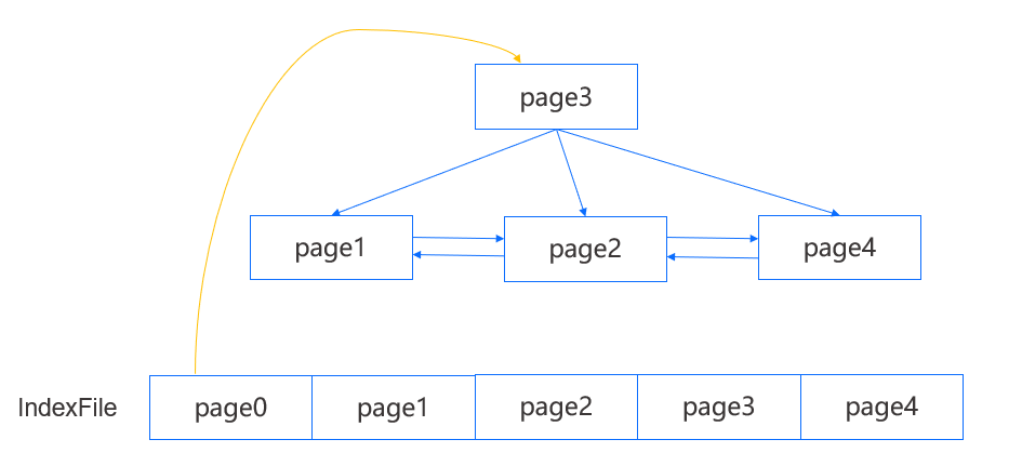
\includegraphics[width=0.6\textwidth]{index-file.png}
  \caption{索引文件图}
\end{figure}

\paragraph{叶子节点}
B+ 树中的每个结点都存放在一个固定大小的 page 中。每个 page 在文件中由 page\_num 唯一标识。结点页都包含一个公共头部（IndexNode），其中记录了结点是否为叶结点（is\_leaf）、当前结点中键的数量（key\_num）以及父结点的页号（parent，为 -1 表示无父结点）。

叶子结点在公共头部之外，还维护了左右兄弟结点的页号（prev\_brother 和 next\_brother），用于支持顺序遍历和范围查询。页中剩余空间按顺序存放键值数据：每个键由索引列的值和对应记录的 RID 组成，Value 同样为 RID。因此，所有索引键及其对应的数据定位信息均存放在叶子结点中，符合 B+ 树“数据集中在叶子结点”的设计特点。

\begin{figure}[H]
  \centering
  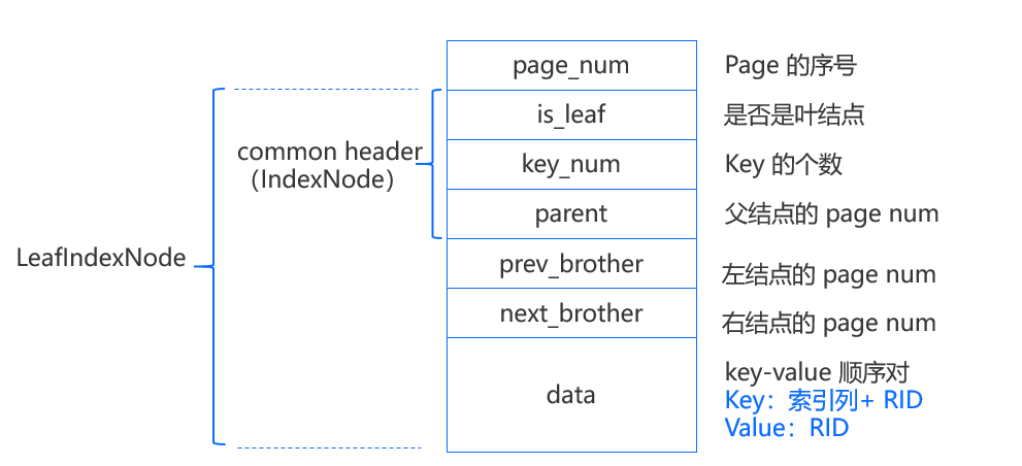
\includegraphics[width=0.6\textwidth]{leaf.png}
  \caption{叶子节点图}
\end{figure}

\paragraph{内部节点}
内部结点和叶结点有两点不同，一个是没有左右结点的 page num；另一个是所存放的值是 page num，也就是标识了子结点的 page 位置。如下图所示，键值对在内部结点是这样表示的，第一个键值对中的键是一个无效数据，真正用于比较的只有 k1 和 k2。

\begin{figure}[H]
  \centering
  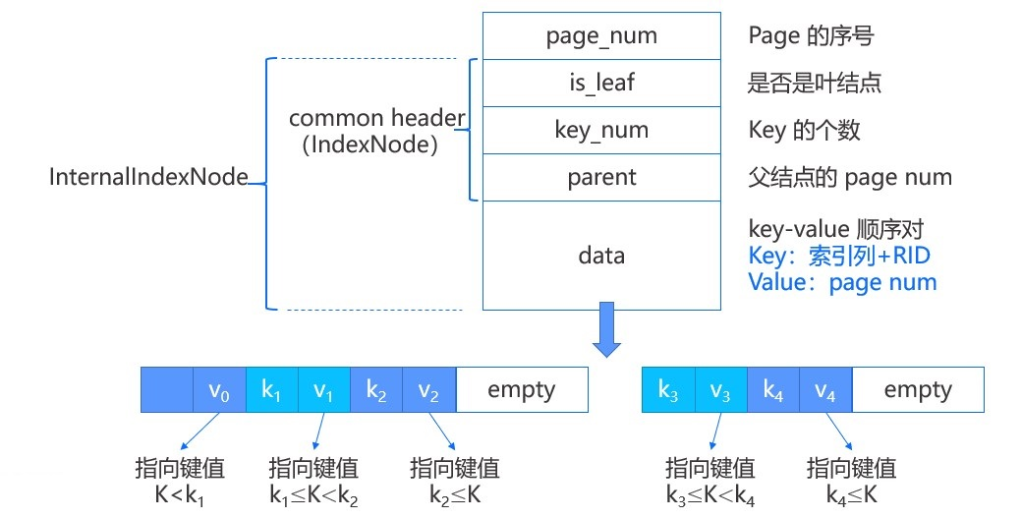
\includegraphics[width=0.6\textwidth]{internal.png}
  \caption{内部节点图}
\end{figure}

\section{具体设计}
\subsection{UPDATE 实现流程}
\begin{enumerate}
    \item \textbf{语法解析} (yacc\_sql.y)：解析表名、赋值列表、条件
    \begin{itemize}
        \item 位置：src/observer/sql/parser/yacc\_sql.y (597-613行)
        \item 功能：将 SQL 语句 \texttt{UPDATE table SET col1=val1, col2=val2 WHERE condition} 解析为表名、赋值列表和条件表达式
    \end{itemize}
    
    \item \textbf{语句创建} (update\_stmt.cpp)：验证表/字段存在，绑定表达式
    
\begin{itemize}
        \item 位置：src/observer/sql/stmt/update\_stmt.cpp (20-154行)
        \item 功能：
        \begin{itemize}
            \item 验证目标表存在
            \item 验证更新字段存在
            \item 绑定 SET 表达式（支持子查询）
            \item 绑定 WHERE 条件表达式
        \end{itemize}
    \end{itemize}
    
    \item \textbf{执行器执行} (update\_executor.cpp)：
    
\begin{itemize}
        \item 位置：src/observer/sql/executor/update\_executor.cpp (35-335行)
        \item 流程：
        \begin{itemize}
            \item 使用 \texttt{RecordScanner} 扫描表记录
            \item 应用 WHERE 条件过滤记录
            \item 对每条匹配记录，计算新字段值
        \end{itemize}
    \end{itemize}
    
    \item \textbf{更新记录} (heap\_table\_engine.cpp)：核心函数 \texttt{update\_record\_with\_trx()}
    
\begin{lstlisting}[language=C++, basicstyle=\footnotesize\ttfamily]
// 更新索引和数据记录的核心函数
RC HeapTableEngine::update_record_with_trx(
    const Record &old_record, 
    const Record &new_record, 
    Trx *trx)
{
    RC rc = RC::SUCCESS;
    
    // 1. 更新索引：先删除旧记录，再插入新记录
    bool *old_bitmap = reinterpret_cast<bool *>(
        const_cast<char *>(old_record.data()) + 
        table_meta_->fields_record_size());
    
    bool *new_bitmap = reinterpret_cast<bool *>(
        const_cast<char *>(new_record.data()) + 
        table_meta_->fields_record_size());
    
    for (Index *index : indexes_) {
        const vector<string> &index_fields = index->index_meta().fields();
        
        // 检查旧值和新值是否包含 NULL（任一字段为 NULL 则跳过索引操作）
        bool old_has_null = false;
        bool new_has_null = false;
        vector<const FieldMeta *> fields_meta;
        
        for (const string &field_name : index_fields) {
            const FieldMeta *field_meta = table_meta_->field(field_name.c_str());
            if (field_meta == nullptr) continue;
            
            fields_meta.push_back(field_meta);
            int bitmap_index = field_meta->field_id() + table_meta_->sys_field_num();
            
            // 检查 NULL 位图
            bool old_is_null = (bitmap_index >= 0 && bitmap_index < table_meta_->field_num()) ? 
                old_bitmap[bitmap_index] : false;
                
            bool new_is_null = (bitmap_index >= 0 && bitmap_index < table_meta_->field_num()) ? 
                new_bitmap[bitmap_index] : false;
            
            if (old_is_null) old_has_null = true;
            if (new_is_null) new_has_null = true;
        }
        
        // 删除旧索引条目（如果非 NULL）
        if (!old_has_null && !fields_meta.empty()) {
            rc = index->delete_entry(old_record.data(), &old_record.rid());
            if (rc != RC::SUCCESS) {
                LOG_WARN("Failed to delete index entry. table=%s, index=%s, rid=%s, rc=%s",
                         table_meta_->name(), index->index_meta().name(), 
                         old_record.rid().to_string().c_str(), strrc(rc));
                return rc;
            }
        }
        
        // 插入新索引条目（如果非 NULL）
        if (!new_has_null && !fields_meta.empty()) {
            // 唯一索引需要先检查键值唯一性
            if (index->index_meta().is_unique()) {
                // 构建复合键（二进制安全）
                int total_key_length = 0;
                for (const FieldMeta *field_meta : fields_meta) {
                    total_key_length += field_meta->len();
                }
                
                char *key_buffer = new char[total_key_length];
                int offset = 0;
                
                // 拼接字段值
                for (const FieldMeta *field_meta : fields_meta) {
                    const char *field_data = new_record.data() + field_meta->offset();
                    memcpy(key_buffer + offset, field_data, field_meta->len());
                    offset += field_meta->len();
                }
                
                // 检查键值是否已存在
                list<RID> existing_rids;
                rc = index->get_entry(key_buffer, total_key_length, existing_rids);
                delete[] key_buffer;
                
                if (rc == RC::SUCCESS && !existing_rids.empty()) {
                    // 排除自身记录（索引字段值未变的情况）
                    bool is_self = false;
                    for (const RID &existing_rid : existing_rids) {
                        if (existing_rid == new_record.rid()) {
                            is_self = true;
                            break;
                        }
                    }
                    
                    // 如果存在其他记录使用相同键值，违反唯一约束
                    if (!is_self) {
                        LOG_WARN("Duplicate key violates unique constraint. table=%s, index=%s", 
                                 table_meta_->name(), index->index_meta().name());
                        return RC::RECORD_DUPLICATE_KEY;
                    }
                }
            }
            
            // 插入新索引条目
            rc = index->insert_entry(new_record.data(), &new_record.rid());
            if (rc != RC::SUCCESS) {
                LOG_WARN("Failed to insert index entry. table=%s, index=%s, rid=%s, rc=%s",
                         table_meta_->name(), index->index_meta().name(), 
                         new_record.rid().to_string().c_str(), strrc(rc));
                return rc;
            }
        }
    }
    
    // 2. 更新数据记录
    rc = record_handler_->delete_record(&old_record.rid());
    if (rc != RC::SUCCESS) {
        LOG_WARN("Failed to delete old record. table=%s, rid=%s, rc=%s",
                 table_meta_->name(), old_record.rid().to_string().c_str(), strrc(rc));
        return rc;
    }
    
    rc = record_handler_->insert_record(
        new_record.data(), 
        new_record.len(), 
        const_cast<RID*>(&new_record.rid()));
    
    if (rc != RC::SUCCESS) {
        LOG_WARN("Failed to insert new record. table=%s, rid=%s, rc=%s",
                 table_meta_->name(), old_record.rid().to_string().c_str(), strrc(rc));
        return rc;
    }
    
    return RC::SUCCESS;
}
    \end{lstlisting}
    
    \textbf{关键设计说明：}
    
\begin{enumerate}
        \item \textbf{NULL 值处理}：
        \begin{itemize}
            \item 遍历索引字段，检查旧值和新值的 NULL 位图
            \item 任一字段为 NULL 则跳过索引操作（SQL 标准允许多个 NULL）
        \end{itemize}
        
        \item \textbf{索引更新策略}：
        
\begin{itemize}
            \item \textcolor{red}{先删除旧索引条目}：若旧值非 NULL，调用 \texttt{index->delete\_entry()}
            \item \textcolor{red}{再插入新索引条目}：若新值非 NULL，先检查唯一性再插入
        \end{itemize}
        
        \item \textbf{唯一性检查}：
        
\begin{itemize}
            \item 构建复合键：拼接所有索引字段的二进制数据
            \item 查询索引获取相同键值的记录列表
            \item 排除自身记录（允许更新非索引字段）
            \item 若存在其他记录，返回 \texttt{RC::RECORD\_DUPLICATE\_KEY}
        \end{itemize}
        
        \item \textbf{数据记录更新}：
        
\begin{itemize}
            \item 先删除旧记录：\texttt{record\_handler\_->delete\_record()}
            \item 再插入新记录：保持相同 RID 实现原地更新
        \end{itemize}
        
        \item \textbf{更新顺序}：
        
\begin{itemize}
            \item \textcolor{blue}{先更新索引再更新数据}：保证一致性
            \item 若先更新数据后更新索引失败，会导致数据与索引不一致
            \item 先更新索引可提前发现唯一性冲突
        \end{itemize}
    \end{enumerate}
    
    \item \textbf{唯一性检查详细流程}
    
\begin{enumerate}
        \item \textbf{构建复合键}：
        \begin{itemize}
            \item 计算总长度：\texttt{total\_key\_length = Σ(field\_meta->len())}
            \item 分配缓冲区：\texttt{char* key\_buffer = new char[total\_key\_length]}
            \item 拼接字段：按索引字段顺序 \texttt{memcpy} 字段数据
            \item \textbf{示例}：索引 \texttt{(name VARCHAR(20), age INT)} → 键结构：\texttt{[20字节name][4字节age]}
        \end{itemize}
        
        \item \textbf{查询索引检查重复}：
        
\begin{itemize}
            \item 调用 \texttt{index->get\_entry(key\_buffer, total\_key\_length, existing\_rids)}
            \item 返回匹配该键的所有 RID 列表
        \end{itemize}
        
        \item \textbf{排除自身记录}：
        
\begin{itemize}
            \item 遍历返回的 RID 列表
            \item 检查是否包含当前记录的 RID
            \item \textbf{场景}：更新非索引字段时（如唯一索引在 \texttt{id}，更新 \texttt{name}）
        \end{itemize}
        
        \item \textbf{冲突检测}：
        
\begin{itemize}
            \item 若存在其他记录的 RID，返回 \texttt{RC::RECORD\_DUPLICATE\_KEY}
            \item 否则允许更新
        \end{itemize}
    \end{enumerate}
    
    \item \textbf{完整流程示例}
    
\begin{itemize}
        \item \textbf{表结构}：
        \begin{lstlisting}[language=SQL]
CREATE TABLE users (
    id INT PRIMARY KEY,
    name VARCHAR(20) UNIQUE,
    age INT
);
        \end{lstlisting}
        
        \item \textbf{更新操作}：\texttt{UPDATE users SET name='Alice' WHERE id=1}
        
\begin{enumerate}
            \item 构建新键：提取 \texttt{name='Alice'} 的二进制数据
            \item 查询索引：\texttt{get\_entry("Alice", ...)} 返回 RID 列表
            \item 排除自身：检查返回列表是否包含 \texttt{id=1} 的 RID
            \item 冲突处理：
            \begin{itemize}
                \item 若包含：允许更新（索引字段值未变）
                \item 若不包含且列表非空：返回 \texttt{RECORD\_DUPLICATE\_KEY}
            \end{itemize}
            \item 插入新键：唯一性检查通过后调用 \texttt{insert\_entry()}
        \end{enumerate}
    \end{itemize}
\end{enumerate}

\subsection{JOIN Table 实现流程}
\begin{enumerate}
    \item \textbf{语法解析} (yacc\_sql.y)
    \begin{itemize}
        \item 位置：src/observer/sql/parser/yacc\_sql.y (912-995行, 998-1030行)
        \item 功能：解析表引用和JOIN条件（如 \texttt{table1 INNER JOIN table2 ON condition}）
        \item 输出：存储到 \texttt{TableReferenceSqlNode}，包含表名、别名和JOIN条件
    \end{itemize}
    
    \item \textbf{语句创建} (select\_stmt.cpp)
    
\begin{itemize}
        \item 位置：src/observer/sql/stmt/select\_stmt.cpp (170-198行, 530-574行)
        \item 流程：
        \begin{itemize}
            \item 解析表引用：验证所有表存在
            \item 收集JOIN条件：遍历 \texttt{table\_references}，收集到 \texttt{all\_join\_conditions}
            \item 创建JOIN过滤器：使用 \texttt{FilterStmt::create} 创建全局JOIN条件过滤器
        \end{itemize}
    \end{itemize}
    
    \item \textbf{逻辑计划生成} (logical\_plan\_generator.cpp)
    
\begin{itemize}
        \item 位置：src/observer/sql/optimizer/logical\_plan\_generator.cpp (111-220行)
        \item 流程：
        \begin{itemize}
            \item 构建JOIN树：为每个表创建 \texttt{TableGetLogicalOperator}
            \item 多表时创建 \texttt{JoinLogicalOperator}
            \item 分配JOIN条件：将条件分配给对应的 \texttt{PredicateLogicalOperator}
        \end{itemize}
    \end{itemize}
    
    \item \textbf{物理计划生成}
    
\begin{itemize}
        \item 位置：src/observer/sql/optimizer/physical\_plan\_generator.cpp
        \item 算法选择：根据会话参数选择 Hash Join 或 Nested Loop Join
        \begin{lstlisting}[language=C++]
// 算法选择逻辑
if (session->hash_join_on() && can_use_hash_join(join_oper)) {
    // 选择 Hash Join
    auto hash_join_oper = make_unique<HashJoinPhysicalOperator>();
    
    // 设置连接字段（等值条件）
    Field left_field, right_field;
    for (auto &expr : join_conditions) {
        if (is_equijoin_condition(expr, left_field, right_field)) {
            hash_join_oper->set_join_fields(left_field, right_field);
            break;
        }
    }
    
    // 设置过滤表达式（包括非等值条件）
    hash_join_oper->set_filter_expressions(predicate_oper->expressions());
    
    oper = std::move(hash_join_oper);
    LOG_INFO("Using Hash Join for this query");
} else {
    // 选择 Nested Loop Join
    auto join_physical_oper = make_unique<NestedLoopJoinPhysicalOperator>();
    oper = std::move(join_physical_oper);
    LOG_INFO("Using Nested Loop Join for this query");
}
        \end{lstlisting}
    \end{itemize}
    
    \item \textbf{Hash Join 实现}
    
\begin{enumerate}
        \item \textbf{构建阶段}：在右表上构建哈希表
        \begin{lstlisting}[language=C++]
void HashJoinPhysicalOperator::build_hash_table()
{
    if (right_join_field_.meta() == nullptr) {
        hash_table_built_ = true;
        return;
    }
    
    while (right_->next() == RC::SUCCESS) {
        // 获取连接键值
        Value join_value;
        get_field_value(right_join_field_, join_value);
        
        // 跳过NULL值
        if (join_value.is_null()) continue;
        
        // 物化右表元组并存入哈希表
        hash_table_[join_value.to_string()].push_back(
            materialize_tuple(right_tuple_)
        );
    }
}
        \end{lstlisting}
        
        \item \textbf{探测阶段}：处理左表行并匹配
        
\begin{lstlisting}[language=C++]
RC HashJoinPhysicalOperator::next()
{
    // 未设置等值键时退化为嵌套循环
    if (left_join_field_.meta() == nullptr) {
        return nested_loop_next();
    }
    
    // 正常Hash Join流程
    if (!current_matches_ || current_match_iter_ == current_matches_->end()) {
        RC rc = probe_hash_table();
        if (rc != RC::SUCCESS) return rc;
    }
    
    // 获取下一个匹配
    right_tuple_ = *current_match_iter_;
    ++current_match_iter_;
    
    // 应用额外过滤条件
    if (!evaluate_filter_conditions(left_tuple_, right_tuple_)) {
        return this->next(); // 跳过不匹配的行
    }
    
    // 组合结果
    joined_tuple_.set_left(left_tuple_);
    joined_tuple_.set_right(right_tuple_);
    
    return RC::SUCCESS;
}
        \end{lstlisting}
        
        \item \textbf{过滤处理}：
        
\begin{lstlisting}[language=C++]
bool HashJoinPhysicalOperator::evaluate_filter_conditions(Tuple *left_tuple, Tuple *right_tuple)
{
    JoinedTuple joined_tuple(left_tuple, right_tuple);
    
    for (auto &expr : filter_expressions_) {
        Value value;
        expr->get_value(joined_tuple, value);
        
        // 任一条件为假则返回false
        if (value.is_null() || !value.get_boolean()) {
            return false;
        }
    }
    return true;
}
        \end{lstlisting}
    \end{enumerate}
    
    \item \textbf{Nested Loop Join 实现}
    
\begin{enumerate}
        \item \textbf{主循环}：
        \begin{lstlisting}[language=C++]
RC NestedLoopJoinPhysicalOperator::next()
{
    while (true) {
        // 如果一轮右表扫描完成，获取下一左表行
        if (round_done_) {
            RC rc = left_next();
            if (rc != RC::SUCCESS) return rc;
        }
        
        // 获取下一右表行
        RC rc = right_next();
        if (rc == RC::RECORD_EOF) {
            round_done_ = true;  // 标记右表扫描完成
            continue;            // 回到循环开始处理下一左表行
        }
        
        // 组合元组并返回
        joined_tuple_.set_left(left_tuple_);
        joined_tuple_.set_right(right_tuple_);
        return RC::SUCCESS;
    }
}
        \end{lstlisting}
        
        \item \textbf{右表控制}：
        
\begin{lstlisting}[language=C++]
RC NestedLoopJoinPhysicalOperator::right_next()
{
    if (round_done_) {
        // 重置右表扫描
        right_->close();
        right_->open(trx_);
        round_done_ = false;
    }
    
    RC rc = right_->next();
    if (rc == RC::RECORD_EOF) {
        round_done_ = true;  // 标记右表扫描完成
    }
    return rc;
}
        \end{lstlisting}
    \end{enumerate}
    
    \item \textbf{JOIN 结果组合}
    
\begin{itemize}
        \item 使用 \texttt{JoinedTuple} 组合左右表元组
        \item 文件：src/observer/sql/expr/tuple.h
        \item 实现原理：
        \begin{lstlisting}[language=C++]
class JoinedTuple : public Tuple {
public:
    JoinedTuple(Tuple *left, Tuple *right) 
        : left_(left), right_(right) {}
    
    // 获取字段值（先左表后右表）
    RC cell_at(int index, Value &cell) override {
        if (index < left_->cell_num()) {
            return left_->cell_at(index, cell);
        }
        return right_->cell_at(index - left_->cell_num(), cell);
    }
    
    int cell_num() const override {
        return left_->cell_num() + right_->cell_num();
    }
    
    // 设置左右表元组
    void set_left(Tuple *left) { left_ = left; }
    void set_right(Tuple *right) { right_ = right; }
    
private:
    Tuple *left_;
    Tuple *right_;
};
        \end{lstlisting}
    \end{itemize}
    
    \item \textbf{核心设计总结}
    
\begin{itemize}
        \item \textcolor{blue}{多表JOIN树}：通过逻辑计划构建JOIN树结构
        \item \textcolor{blue}{算法自适应}：
        \begin{itemize}
            \item Hash Join：适用于等值连接，O(M+N)时间复杂度
            \item Nested Loop Join：通用算法，支持任意连接条件
        \end{itemize}
        \item \textcolor{blue}{NULL处理}：连接键为NULL时不参与匹配
        \item \textcolor{blue}{统一接口}：使用 \texttt{JoinedTuple} 透明访问多表字段
    \end{itemize}
\end{enumerate}

\subsubsection*{JOIN 执行流程示意图}
\begin{center}
\begin{tikzpicture}[node distance=2cm, auto]
    \node (parse) [rectangle, draw, text width=3cm, text centered] {语法解析 \\ (yacc\_sql.y)};
    \node (stmt) [rectangle, draw, below of=parse, text width=3cm, text centered] {语句创建 \\ (select\_stmt.cpp)};
    \node (logical) [rectangle, draw, below of=stmt, text width=3cm, text centered] {逻辑计划生成 \\ (logical\_plan\_generator.cpp)};
    \node (physical) [rectangle, draw, below of=logical, text width=3cm, text centered] {物理计划生成};
    \node (hash) [rectangle, draw, right of=physical, xshift=3cm, text width=2.5cm, text centered] {Hash Join};
    \node (nested) [rectangle, draw, left of=physical, xshift=-3cm, text width=2.5cm, text centered] {Nested Loop Join};
    \node (result) [rectangle, draw, below of=physical, text width=3cm, text centered] {结果组合 \\ (JoinedTuple)};
    
    \draw [->] (parse) -- (stmt);
    \draw [->] (stmt) -- (logical);
    \draw [->] (logical) -- (physical);
    \draw [->] (physical) -- node[above] {等值条件} (hash);
    \draw [->] (physical) -- node[above] {其他条件} (nested);
    \draw [->] (hash) |- (result);
    \draw [->] (nested) |- (result);
\end{tikzpicture}
\end{center}

\subsubsection*{Hash Join vs Nested Loop Join 对比}
\begin{table}[h]
\centering
\begin{tabular}{|l|c|c|}
\hline
\textbf{特性} & \textbf{Hash Join} & \textbf{Nested Loop Join} \\
\hline
适用条件 & 等值连接 & 任意连接条件 \\
时间复杂度 & O(M + N) & O(M × N) \\
内存使用 & 高（需建哈希表） & 低（流式处理） \\
NULL处理 & 跳过NULL键 & 处理NULL键 \\
实现复杂度 & 中等 & 简单 \\
\hline
\end{tabular}
\caption{JOIN算法特性对比}
\end{table}

\subsection{复合索引实现流程}
\begin{enumerate}
    \item \textbf{语法解析} (yacc\_sql.y)
    \begin{itemize}
        \item 位置：src/observer/sql/parser/yacc\_sql.y (366-385行)
        \item 功能：解析多字段索引（如 \texttt{CREATE INDEX idx ON table(id, name)}）
        \item 输出：字段名列表 \texttt{["id", "name"]}
    \end{itemize}
    
    \item \textbf{语句创建} (create\_index\_stmt.cpp)
    
\begin{itemize}
        \item 位置：src/observer/sql/stmt/create\_index\_stmt.cpp (24-68行)
        \item 流程：
        \begin{itemize}
            \item 验证所有字段存在
            \item 收集 \texttt{FieldMeta} 指针
            \item 处理唯一性约束标志
        \end{itemize}
    \end{itemize}
    
    \item \textbf{索引元数据} (index\_meta.cpp)
    
\begin{itemize}
        \item 位置：src/observer/storage/index/index\_meta.cpp (42-65行)
        \item 功能：\texttt{IndexMeta} 存储字段名列表 \texttt{fields\_}，支持单字段和多字段索引
    \end{itemize}
    
    \item \textbf{索引创建} (heap\_table\_engine.cpp)
    
\begin{itemize}
        \item 位置：src/observer/storage/table/heap\_table\_engine.cpp
        \item 流程：
        \begin{itemize}
            \item 唯一性检查：扫描记录，构建复合键检查重复
            \item 创建B+树索引文件（键类型为 \texttt{CHARS}，长度为所有字段长度之和）
            \item 填充索引：扫描所有记录，插入复合键
        \end{itemize}
    \end{itemize}
    
    \item \textbf{复合键构建}
    
\begin{itemize}
        \item 位置：\texttt{BplusTreeIndex::build\_composite\_key}
        \item 功能：按索引字段顺序拼接字段的二进制数据
        \begin{lstlisting}[language=C++]
// 构建复合键的核心代码
int total_length = 0;
for (const FieldMeta *field_meta : fields_meta_) {
    total_length += field_meta->len(); // 累加字段长度
}

char *key_buffer = new char[total_length];
int offset = 0;

// 按顺序拼接字段数据
for (const FieldMeta *field_meta : fields_meta_) {
    const char *field_data = record + field_meta->offset();
    memcpy(key_buffer + offset, field_data, field_meta->len());
    offset += field_meta->len();
}
        \end{lstlisting}
        \item \textbf{设计要点}：
        
\begin{itemize}
            \item 使用字段的固定长度 \texttt{field\_meta->len()}
            \item 字符字段不足时用原记录填充保证键长度恒定
            \item 复合键为"字段字节段的顺序拼接"，B+树视为固定长度字节流
        \end{itemize}
    \end{itemize}
    
    \item \textbf{索引扫描的前缀扩展}
    
\begin{itemize}
        \item 位置：\texttt{BplusTreeIndex::open} 中的范围准备逻辑
        \item 功能：当查询键长度小于完整复合键时自动补全
        \begin{lstlisting}[language=C++]
// 左边界补最小值
if (left_key && left_len < full_key_length) {
    for (int j = start_field_idx; j < fields_meta_.size(); j++) {
        const FieldMeta *field_meta = fields_meta_[j];
        switch (field_meta->type()) {
            case INTS:  fill_value(expanded_left_key + offset, INT_MIN); break;
            case FLOATS: fill_value(expanded_left_key + offset, -FLT_MAX); break;
            default:    memset(expanded_left_key + offset, 0, field_meta->len());
        }
        offset += field_meta->len();
    }
    final_left_key = expanded_left_key;
    final_left_len = full_key_length;
}

// 右边界补最大值
if (right_key && right_len < full_key_length) {
    for (int j = start_field_idx; j < fields_meta_.size(); j++) {
        const FieldMeta *field_meta = fields_meta_[j];
        switch (field_meta->type()) {
            case INTS:  fill_value(expanded_right_key + offset, INT_MAX); break;
            case FLOATS: fill_value(expanded_right_key + offset, FLT_MAX); break;
            default:    memset(expanded_right_key + offset, 0xFF, field_meta->len());
        }
        offset += field_meta->len();
    }
    final_right_key = expanded_right_key;
    final_right_len = full_key_length;
}
        \end{lstlisting}
        \item \textbf{作用}：如查询 \texttt{id=3} 时扩展为 \texttt{[3+min, 3+max]}，扫描所有 \texttt{id=3} 的记录
    \end{itemize}
    
    \item \textbf{索引操作}
    
\begin{itemize}
        \item 位置：\texttt{BplusTreeIndex::insert\_entry}, \texttt{delete\_entry}, \texttt{get\_entry}
        \item 统一接口：
        \begin{lstlisting}[language=C++]
RC BplusTreeIndex::insert_entry(const char *record, const RID *rid) {
    char key_buf[key_len_];
    build_composite_key(record, key_buf); // 构建复合键
    return index_handler_.insert_entry(key_buf, rid); // 调用B+树插入
}

RC BplusTreeIndex::delete_entry(const char *record, const RID *rid) {
    char key_buf[key_len_];
    build_composite_key(record, key_buf);
    return index_handler_.delete_entry(key_buf, rid);
}

RC BplusTreeIndex::get_entry(const char *key, int key_len, list<RID> &rids) {
    return index_handler_.get_entry(key, key_len, rids);
}
        \end{lstlisting}
        \item \textbf{更新场景}：
        
\begin{itemize}
            \item 先 \texttt{delete\_entry} 旧键
            \item 再 \texttt{insert\_entry} 新键
            \item 唯一索引会先 \texttt{get\_entry} 查重
        \end{itemize}
    \end{itemize}
\end{enumerate}

\begin{table}[h]
\centering
\begin{tabular}{|c|c|c|}
\hline
\textbf{查询条件} & \textbf{扩展后左边界} & \textbf{扩展后右边界} \\
\hline
\texttt{id=3} & \texttt{3 + INT\_MIN} & \texttt{3 + INT\_MAX} \\
\hline
\texttt{name='Tom'} & \texttt{'Tom' + \textbackslash{}0} & \texttt{'Tom' + \textbackslash{}xFF} \\
\hline
\texttt{id>3 AND name<'Lee'} & \texttt{3 + min + 'Lee' + min} & \texttt{3 + max + 'Lee' + max} \\
\hline
\end{tabular}
\caption{复合索引前缀扩展规则}
\end{table}

\subsection{四、UNIQUE 索引实现流程}
UNIQUE 索引用于保证索引键的唯一性（NULL 值除外），其实现流程涵盖语法解析、元数据存储、创建/插入/更新阶段的唯一性检查，以及 NULL 值处理等环节。

\begin{enumerate}
    \item \textbf{语法解析} (yacc\_sql.y)
    \begin{itemize}
        \item \textbf{位置}：src/observer/sql/parser/yacc\_sql.y (356-365行, 376-385行)
        \item \textbf{功能}：解析\texttt{CREATE UNIQUE INDEX}语句时，识别\texttt{UNIQUE}关键字并设置索引的\texttt{is\_unique}标志为\texttt{true}。
        \item \textbf{语法规则示例}：
        \begin{lstlisting}[language=SQL]
CREATE UNIQUE INDEX idx_user_id ON users(id); -- 唯一索引
CREATE INDEX idx_user_name ON users(name);     -- 普通索引
        \end{lstlisting}
        \item \textbf{解析逻辑}：在 Yacc 语法规则中，\texttt{UNIQUE}作为可选关键字匹配，若存在则将\texttt{CreateIndexStmt}的\texttt{is\_unique}属性设为\texttt{true}（对应代码中\texttt{stmt->set\_is\_unique(true)}）。
    \end{itemize}

    \item \textbf{元数据存储} (index\_meta.cpp/h)
    
\begin{itemize}
        \item \textbf{位置}：
        \begin{itemize}
            \item 定义：src/observer/storage/index/index\_meta.h (47行, 59行)
            \item 实现：src/observer/storage/index/index\_meta.cpp (27-40行)
        \end{itemize}
        \item \textbf{功能}：\texttt{IndexMeta}类通过\texttt{is\_unique\_}成员变量存储索引的唯一性标志，支持获取和设置操作。
        \item \textbf{代码片段}：
        
\begin{lstlisting}[language=C++]
// index_meta.h（定义）
class IndexMeta {
private:
    bool is_unique_; // 唯一索引标志（true表示唯一）
public:
    bool is_unique() const { return is_unique_; } // 获取唯一性状态
    void set_is_unique(bool is_unique) { is_unique_ = is_unique; } // 设置唯一性状态
};

// index_meta.cpp（实现）
IndexMeta::IndexMeta(const char* name, const std::vector<const FieldMeta*>& fields, bool is_unique)
    : name_(name), fields_(fields), is_unique_(is_unique) {}
        \end{lstlisting}
    \end{itemize}

    \item \textbf{创建索引时的唯一性检查}
    
\begin{itemize}
        \item \textbf{逻辑}：创建唯一索引前，通过\texttt{RecordScanner}全表遍历，构建索引键并使用哈希表\texttt{key\_to\_rid}查重。若发现重复键，立即返回\texttt{RC::RECORD\_DUPLICATE\_KEY}，终止索引创建。
        \item \textbf{NULL 处理}：若索引字段包含\texttt{NULL}（通过记录的\texttt{NULL}位图判断），则跳过该记录的唯一性检查（允许多个\texttt{NULL}）。
        \item \textbf{代码片段}（heap\_table\_engine.cpp）：
        \begin{lstlisting}[language=C++]
// 创建唯一索引时的全表唯一性检查
std::unordered_map<std::string, RID> key_to_rid; // 哈希表：键→RID
RecordScanner check_scanner(table_meta_, record_handler_);
RC rc = check_scanner.open();
if (OB_FAIL(rc)) return rc;

while (OB_SUCC(rc = check_scanner.next(record))) {
    // 1. 检查索引字段是否为NULL（通过 bitmap 判断）
    bool is_field_null = false;
    const char* bitmap = record.data() + table_meta_->fields_record_size(); // NULL位图位置
    for (const FieldMeta* field : index_meta.fields()) {
        int field_id = field->field_id();
        if (bitmap[field_id / 8] & (1 << (field_id % 8))) { // 位图位为1表示NULL
            is_field_null = true;
            break;
        }
    }
    if (is_field_null) continue; // NULL值跳过检查

    // 2. 构建索引键（复合键为字段字节拼接）
    std::string key_str;
    for (const FieldMeta* field : index_meta.fields()) {
        const char* field_data = record.data() + field->offset();
        key_str.append(field_data, field->len()); // 拼接字段字节
    }

    // 3. 查重：若键已存在，返回重复错误
    if (key_to_rid.find(key_str) != key_to_rid.end()) {
        check_scanner.close();
        return RC::RECORD_DUPLICATE_KEY;
    }
    key_to_rid[key_str] = record.rid(); // 键→RID映射
}

check_scanner.close();
        \end{lstlisting}
    \end{itemize}

    \item \textbf{插入记录时的唯一性检查}
    
\begin{itemize}
        \item \textbf{逻辑}：插入记录前，对每个唯一索引，构建索引键并查询索引（\texttt{index->get\_entry}）。若索引中存在相同键，返回\texttt{RC::RECORD\_DUPLICATE\_KEY}，拒绝插入。
        \item \textbf{NULL 处理}：若索引键包含\texttt{NULL}，跳过检查（允许多个\texttt{NULL}）。
        \item \textbf{代码片段}（heap\_table\_engine.cpp）：
        \begin{lstlisting}[language=C++]
// 插入记录时的唯一索引检查
for (Index* index : indexes_) {
    if (!index->index_meta().is_unique()) continue; // 非唯一索引跳过

    // 1. 检查索引字段是否为NULL（通过 bitmap 判断）
    bool is_field_null = false;
    const char* bitmap = record.data() + table_meta_->fields_record_size();
    for (const FieldMeta* field : index->index_meta().fields()) {
        int field_id = field->field_id();
        if (bitmap[field_id / 8] & (1 << (field_id % 8))) {
            is_field_null = true;
            break;
        }
    }
    if (is_field_null) continue;

    // 2. 构建复合键
    int total_len = 0;
    for (const FieldMeta* field : index->index_meta().fields()) {
        total_len += field->len();
    }
    char* key_buffer = new char[total_len];
    int offset = 0;
    for (const FieldMeta* field : index->index_meta().fields()) {
        const char* field_data = record.data() + field->offset();
        memcpy(key_buffer + offset, field_data, field->len());
        offset += field->len();
    }

    // 3. 查询索引：是否存在相同键
    std::list<RID> existing_rids;
    RC rc = index->get_entry(key_buffer, total_len, existing_rids);
    delete[] key_buffer;
    if (rc == RC::SUCCESS && !existing_rids.empty()) {
        return RC::RECORD_DUPLICATE_KEY; // 存在重复键，拒绝插入
    }
}
        \end{lstlisting}
    \end{itemize}

    \item \textbf{更新记录时的唯一性检查}
    
\begin{itemize}
        \item \textbf{逻辑}：更新记录时，需删除旧键并插入新键。插入新键前，对每个唯一索引进行检查：
        \begin{enumerate}
            \item 构建新键；
            \item 查询索引是否存在相同键；
            \item 若存在，排除当前记录自身（\texttt{existing\_rid == new\_record.rid()}），若仍有其他记录，则返回重复错误。
        \end{enumerate}
        \item \textbf{代码片段}（heap\_table\_engine.cpp）：
        
\begin{lstlisting}[language=C++]
// 更新记录时的唯一索引检查（插入新键前）
for (Index* index : indexes_) {
    if (!index->index_meta().is_unique()) continue;

    // 1. 检查新记录的索引字段是否为NULL（通过 bitmap 判断）
    bool new_has_null = false;
    const char* new_bitmap = new_record.data() + table_meta_->fields_record_size();
    for (const FieldMeta* field : index->index_meta().fields()) {
        int field_id = field->field_id();
        if (new_bitmap[field_id / 8] & (1 << (field_id % 8))) {
            new_has_null = true;
            break;
        }
    }
    if (new_has_null) continue;

    // 2. 构建新复合键
    int total_key_length = 0;
    for (const FieldMeta* field : index->index_meta().fields()) {
        total_key_length += field->len();
    }
    char* key_buffer = new char[total_key_length];
    int offset = 0;
    for (const FieldMeta* field : index->index_meta().fields()) {
        const char* field_data = new_record.data() + field->offset();
        memcpy(key_buffer + offset, field_data, field->len());
        offset += field->len();
    }

    // 3. 查询索引是否存在相同键
    std::list<RID> existing_rids;
    RC rc = index->get_entry(key_buffer, total_key_length, existing_rids);
    delete[] key_buffer;
    if (rc == RC::SUCCESS && !existing_rids.empty()) {
        // 排除当前记录自身（索引字段未变更的情况）
        bool is_self = false;
        for (const RID& rid : existing_rids) {
            if (rid == new_record.rid()) {
                is_self = true;
                break;
            }
        }
        if (!is_self) {
            return RC::RECORD_DUPLICATE_KEY; // 存在其他记录的重复键
        }
    }
}
        \end{lstlisting}
        \item \textbf{排除自身的必要性}：更新非索引字段时（如唯一索引在\texttt{id}，更新\texttt{name}），索引键未变，查询会返回当前记录自身，需排除以避免误判冲突。
    \end{itemize}

    \item \textbf{NULL 值处理}
    
\begin{itemize}
        \item \textbf{逻辑}：遵循 SQL 标准（ISO/IEC 9075），\texttt{NULL}视为“未知”，不与任何值相等（包括自身）。因此，唯一索引允许多个\texttt{NULL}值（\texttt{NULL}不会被视为重复）。
        \item \textbf{实现位置}：src/observer/storage/table/heap\_table\_engine.cpp (309-320行, 523行)
    \end{itemize}
\end{enumerate}

\subsubsection*{核心设计要点}
\begin{itemize}
    \item \textbf{三阶段一致性保障}：
    \begin{enumerate}
        \item 创建时：全表扫描检查历史数据重复；
        \item 插入时：实时查询索引检查新键冲突；
        \item 更新时：排除自身后检查新键冲突。
    \end{enumerate}
    \item \textbf{SQL 标准兼容}：严格支持\texttt{NULL}值语义，允许多个\texttt{NULL}共存。
    \item \textbf{性能优化}：
    
\begin{itemize}
        \item 创建时全表扫描仅执行一次；
        \item 插入/更新时通过索引查询（\texttt{O(log n)}）而非全表扫描；
        \item 复合键使用二进制拼接，哈希表/索引查询高效。
    \end{itemize}
    \item \textbf{冲突处理}：通过返回\texttt{RC::RECORD\_DUPLICATE\_KEY}明确拒绝重复键，保证数据一致性。
\end{itemize}

\subsection{五、子查询实现流程}
子查询是 SQL 中嵌套在其他查询内部的查询语句，支持在 WHERE 条件、UPDATE SET 子句、比较表达式和 IN/NOT IN 等场景中使用。以下是子查询在 MiniOB 中的实现流程：

\begin{enumerate}
    \item \textbf{语法解析} (yacc\_sql.y)
    \begin{itemize}
        \item \textbf{位置}：src/observer/sql/parser/yacc\_sql.y (601-651行, 1151-1211行)
        \item \textbf{功能}：解析形如 \texttt{(SELECT ...)} 的子查询结构，创建 \texttt{subquery\_stmt} 节点，并用 \texttt{SubqueryExpr} 包装解析树。
        \item \textbf{支持场景}：
        \begin{itemize}
            \item WHERE 条件中的子查询：\texttt{SELECT * FROM t1 WHERE id IN (SELECT id FROM t2)}
            \item UPDATE SET 表达式：\texttt{UPDATE t1 SET col = (SELECT MAX(val) FROM t2)}
            \item 比较表达式：\texttt{SELECT * FROM t1 WHERE col > (SELECT AVG(col) FROM t2)}
            \item IN/NOT IN 子句
        \end{itemize}
    \end{itemize}

    \item \textbf{表达式绑定} (select\_stmt.cpp)
    
\begin{itemize}
        \item \textbf{位置}：src/observer/sql/stmt/select\_stmt.cpp (452-500行)
        \item \textbf{流程}：
        \begin{enumerate}
            \item 为 \texttt{SubqueryExpr} 创建 \texttt{SelectStmt} 对象
            \item 传递表上下文：子查询可访问外层查询的表（支持相关子查询）
            \item 合法性检查：确保标量子查询只返回单个属性
            \item 绑定子查询内部的表达式
        \end{enumerate}
        \item \textbf{代码片段}：
        
\begin{lstlisting}[language=C++]
// 创建子查询 SelectStmt
if (expr->type() == ExprType::SUB_QUERY) {
    SubqueryExpr *subquery_expr = static_cast<SubqueryExpr*>(expr.get());
    RC rc = SelectStmt::create(db, 
                              *subquery_expr->sub_query_sn(), 
                              stmt, 
                              subquery_expr->stmt_ref());
    if (rc != RC::SUCCESS) return rc;
    
    // 检查标量子查询只返回单列
    if (subquery_expr->stmt()->projects().size() != 1) {
        return RC::SUBQUERY_TOO_MANY_COLUMNS;
    }
}
        \end{lstlisting}
    \end{itemize}

    \item \textbf{逻辑计划生成}
    
\begin{itemize}
        \item \textbf{位置}：LogicalPlanGenerator
        \item \textbf{功能}：为子查询生成逻辑算子树，并存储到 \texttt{SubqueryExpr} 中
        \item \textbf{接口设计}：
        \begin{lstlisting}[language=C++]
class SubqueryExpr {
private:
    std::unique_ptr<LogicalOperator> logical_operator_;
    std::unique_ptr<PhysicalOperator> physical_operator_;
public:
    void set_logical_operator(std::unique_ptr<LogicalOperator> logical_operator) {
        logical_operator_ = std::move(logical_operator);
    }
    void set_physical_operator(std::unique_ptr<PhysicalOperator> physical_operator) {
        physical_operator_ = std::move(physical_operator);
    }
};
        \end{lstlisting}
        \item \textbf{流程}：表达式绑定后，调用 \texttt{LogicalPlanGenerator} 生成子查询的逻辑算子树，并通过 \texttt{set\_logical\_operator()} 存储。
    \end{itemize}

    \item \textbf{物理计划生成}
    
\begin{itemize}
        \item \textbf{TableGet 场景}：
        \begin{lstlisting}[language=C++]
// 处理比较表达式中的子查询
if (comparison_expr->left()->type() == ExprType::SUB_QUERY) {
    auto sub_query_expr = static_cast<SubqueryExpr*>(comparison_expr->left().get());
    unique_ptr<PhysicalOperator> subquery_phy_oper;
    RC rc = create(*sub_query_expr->logical_operator(), 
                  subquery_phy_oper, 
                  session);
    sub_query_expr->set_physical_operator(std::move(subquery_phy_oper));
}
// 右子树同理
        \end{lstlisting}
        
        \item \textbf{Predicate 场景}：
        
\begin{lstlisting}[language=C++]
// 为过滤条件中的子查询生成物理算子
if (comparison_expr->left()->type() == ExprType::SUB_QUERY) {
    auto sub_query_expr = static_cast<SubqueryExpr*>(expr.get());
    if (session) sub_query_expr->set_trx(session->current_trx());
    unique_ptr<PhysicalOperator> subquery_phy_oper;
    RC rc = create(*sub_query_expr->logical_operator(), 
                  subquery_phy_oper, 
                  session);
    sub_query_expr->set_physical_operator(std::move(subquery_phy_oper));
}
        \end{lstlisting}
        \item \textbf{说明}：物理算子生成后存储到 \texttt{SubqueryExpr} 中，供执行阶段使用。
    \end{itemize}

    \item \textbf{执行阶段}
    
\begin{itemize}
        \item \textbf{流程}：
        \begin{enumerate}
            \item 打开物理算子（传入外层元组指针）
            \item 获取首行首列值
            \item 检查行数：多行报错，无行返回 NULL
            \item 关闭物理算子
        \end{enumerate}
        \item \textbf{代码片段}：
        
\begin{lstlisting}[language=C++]
RC SubqueryExpr::get_value(Tuple *outer_tuple, Value &value) {
    // 1. 打开物理算子（传入外层元组）
    RC rc = open_physical_operator(outer_tuple);
    if (rc != RC::SUCCESS) return rc;
    
    // 2. 获取首行
    rc = physical_operator_->next();
    if (rc == RC::RECORD_EOF) { // 无结果返回NULL
        value.set_null();
        close_physical_operator();
        return RC::SUCCESS;
    }
    
    // 3. 读取第一列
    Tuple *sub_t = physical_operator_->current_tuple();
    rc = sub_t->cell_at(0, value);
    
    // 4. 检查是否多行
    RC next_rc = physical_operator_->next();
    if (next_rc == RC::SUCCESS) {
        close_physical_operator();
        return RC::SUBQUERY_MULTIPLE_ROWS; // 多行报错
    }
    
    // 5. 关闭算子
    close_physical_operator();
    return rc;
}
        \end{lstlisting}
    \end{itemize}

    \item \textbf{相关子查询支持}
    
\begin{itemize}
        \item \textbf{机制}：通过 \texttt{set\_outer\_tuple()} 传递外层元组指针
        \item \textbf{代码实现}：
        \begin{lstlisting}[language=C++]
// 打开子查询物理算子时传递外层元组
RC open_physical_operator(Tuple *outer_tuple) {
    physical_operator_->set_outer_tuple(outer_tuple);
    return physical_operator_->open(trx_);
}
        \end{lstlisting}
    \end{itemize}

    \item \textbf{绑定阶段合法性检查}
    
\begin{itemize}
        \item \textbf{SELECT 场景}：
        \begin{lstlisting}[language=C++]
if (condition.left_expr->type() == ExprType::SUB_QUERY) {
    SelectStmt::create(db, subquery_sn->selection, stmt);
    check_sub_select_legal(subquery_expr->stmt()); // 检查单列
}
        \end{lstlisting}
        
        \item \textbf{UPDATE 场景}：
        
\begin{lstlisting}[language=C++]
if (value_expr->type() == ExprType::SUB_QUERY) {
    SelectStmt::create(db, subquery_sn->selection, nullptr); // 无外层表
    Stmt::check_sub_select_legal(subquery_expr->stmt());
}
        \end{lstlisting}
        \item \textbf{规则}：
        
\begin{itemize}
            \item 标量子查询必须返回单列
            \item UPDATE SET 中的子查询不能引用外层表
        \end{itemize}
    \end{itemize}

    \item \textbf{UPDATE 中的子查询}
    
\begin{itemize}
        \item \textbf{位置}：src/observer/sql/stmt/update\_stmt.cpp (55-83行, 105-127行)
        \item \textbf{流程}：
        \begin{enumerate}
            \item 解析 SET 子句中的子查询表达式
            \item 创建 \texttt{SelectStmt}
            \item 检查子查询是否只返回单列
            \item 绑定表达式
        \end{enumerate}
    \end{itemize}
\end{enumerate}

\subsubsection*{设计要点总结}
\begin{itemize}
    \item \textbf{分层处理}：语法解析 → 表达式绑定 → 逻辑计划 → 物理计划 → 执行
    \item \textbf{表达式封装}：通过 \texttt{SubqueryExpr} 统一管理子查询的逻辑和物理算子
    \item \textbf{相关子查询}：通过 \texttt{outer\_tuple} 机制实现外层数据传递
    \item \textbf{执行优化}：惰性执行（需要时才打开算子）
    \item \textbf{安全机制}：
    \begin{itemize}
        \item 标量子查询强制单列检查
        \item UPDATE SET 子查询禁止引用外层表
        \item 多行结果自动报错
    \end{itemize}
\end{itemize}

\subsection{六、ALIAS（别名）实现流程}
别名机制用于为表或字段提供临时名称，提升查询可读性和灵活性。MiniOB 支持表别名和字段别名，并处理了多层嵌套查询中的别名遮蔽问题。

\begin{enumerate}
    \item \textbf{语法解析} (yacc\_sql.y)
    \begin{itemize}
        \item \textbf{位置}：src/observer/sql/parser/yacc\_sql.y (772-812行, 900行)
        \item \textbf{功能}：
        \begin{itemize}
            \item 表别名：解析 \texttt{table AS alias} 或 \texttt{table alias} 结构，存储到 \texttt{RelationSqlNode.alias}
            \item 字段别名：解析 \texttt{expression AS alias} 或 \texttt{expression alias} 结构，调用 \texttt{expression->set\_alias()}
        \end{itemize}
    \end{itemize}

    \item \textbf{表别名处理}
    
\begin{itemize}
        \item \textbf{收集与映射}：
        \begin{itemize}
            \item 构建 \texttt{table\_alias\_map} 映射：别名 → 真实表名
            \item 检查重复：同一查询层内不允许别名指向不同表
        \end{itemize}
        \item \textbf{代码实现}：
        
\begin{lstlisting}[language=C++]
// 构建别名映射并检查重复
std::unordered_map<std::string, std::string> table_alias_map;
for (const auto &a : select_sql.ALIASES) {
    if (visible_tables.count(a.name) == 0) continue; // 跳过外层表
    if (table_alias_map.find(a.alias) != table_alias_map.end() && 
        table_alias_map[a.alias] != a.name) {
        return RC::INVALID_ARGUMENT; // 别名冲突
    }
    table_alias_map[a.alias] = a.name;
}

// 补充JOIN表的别名
for (const auto &tr : select_sql.table_references) {
    if (!tr.alias.empty() && visible_tables.count(tr.table_name)) {
        table_alias_map[tr.alias] = tr.table_name;
    }
}
        \end{lstlisting}
        \item \textbf{注册与传递}：
        
\begin{lstlisting}[language=C++]
// 注册到绑定上下文
for (const auto &kv : table_alias_map) {
    binder_context.add_table_alias(kv.first.c_str(), table);
}

// 向子查询传递别名映射
if (name2alias) name2alias->insert({real_table, alias});
if (alias2name) alias2name->insert({alias, real_table});
        \end{lstlisting}
        \item \textbf{遮蔽规则}：本层别名可遮蔽外层同名别名
    \end{itemize}

    \item \textbf{字段别名处理}
    
\begin{itemize}
        \item \textbf{收集}：构建 \texttt{field\_alias\_map}（别名 → 原始字段名）
        \item \textbf{限制}：星号(\texttt{*})不允许带别名
        \item \textbf{代码实现}：
        \begin{lstlisting}[language=C++]
std::unordered_map<std::string, std::string> field_alias_map;
for (auto *expr : select_sql.expressions) {
    if (expr->type() == ExprType::STAR) {
        if (static_cast<StarExpr*>(expr)->has_alias()) {
            return RC::INVALID_ARGUMENT; // 星号禁止别名
        }
    } else if (expr->has_alias()) {
        field_alias_map[expr->alias()] = expr->name();
    }
}
        \end{lstlisting}
        \item \textbf{用途}：ORDER BY/GROUP BY 子句可引用字段别名
    \end{itemize}

    \item \textbf{别名解析} (select\_stmt.cpp)
    
\begin{itemize}
        \item \textbf{位置}：src/observer/sql/stmt/select\_stmt.cpp (343-380行)
        \item \textbf{流程}：
        \begin{enumerate}
            \item 表别名解析：将 \texttt{UnboundFieldExpr} 中的别名映射到真实表名
            \item 字段别名解析：在 ORDER BY 等子句中解析字段别名
            \item 默认绑定：单表查询时未指定表名的字段自动绑定
        \end{enumerate}
    \end{itemize}

    \item \textbf{别名绑定} (expression\_binder.cpp)
    
\begin{itemize}
        \item \textbf{位置}：src/observer/sql/parser/expression\_binder.cpp (23-39行)
        \item \textbf{机制}：
        \begin{itemize}
            \item 表别名查找：\texttt{BinderContext::find\_table(alias)}
            \item 字段别名查找：通过 \texttt{field\_alias\_map} 映射
        \end{itemize}
        \item \textbf{查找顺序}：
        
\begin{enumerate}
            \item 本层表别名
            \item 本层表名
            \item 外层别名（支持相关子查询）
        \end{enumerate}
    \end{itemize}

    \item \textbf{别名传递与遮蔽}
    
\begin{itemize}
        \item \textbf{传递机制}：通过 \texttt{name2alias/alias2name} 映射向子查询传递别名
        \item \textbf{遮蔽规则}：子查询可访问外层别名，但本层别名优先
        \item \textbf{代码实现}：
        \begin{lstlisting}[language=C++]
// 绑定字段表达式时的别名处理
if (field_expr->table_name()) {
    auto iter = table_alias_map.find(table_name);
    if (iter != table_alias_map.end()) { // 本层别名
        field_expr->set_real_table(iter->second);
    } else if (visible_tables.count(table_name)) { // 本层表名
        // 直接使用
    } else { // 尝试外层
        Table *outer_table = outer_context->find_table(table_name);
        if (outer_table) field_expr->set_real_table(outer_table->name());
    }
}
        \end{lstlisting}
    \end{itemize}

    \item \textbf{别名输出}
    
\begin{itemize}
        \item \textbf{位置}：src/observer/sql/operator/project\_physical\_operator.cpp (82-84行)
        \item \textbf{机制}：Project 算子使用字段别名构建输出 Schema
        \item \textbf{代码实现}：
        \begin{lstlisting}[language=C++]
// 构建输出Schema
for (auto &expr : expressions_) {
    TupleCellSpec spec(expr->name().c_str(), expr->alias().c_str());
    tuple_schema_.add_cell_spec(spec);
}
        \end{lstlisting}
        \item \textbf{效果}：查询结果列名优先使用字段别名
        
\begin{center}
        \begin{tabular}{|c|c|}
            \hline
            \textbf{原始列名} & \textbf{输出列名} \\
            \hline
            \texttt{salary} & \texttt{annual\_income} \\
            \hline
            \texttt{name} & \texttt{employee\_name} \\
            \hline
        \end{tabular}
        \end{center}
    \end{itemize}
\end{enumerate}

\subsubsection*{别名处理流程图}
\begin{center}
\begin{tikzpicture}[node distance=1.5cm]
    \node (parse) [rectangle, draw] {语法解析};
    \node (collect) [rectangle, draw, below of=parse] {别名收集};
    \node (resolve) [rectangle, draw, below of=collect] {别名解析};
    \node (bind) [rectangle, draw, below of=resolve] {表达式绑定};
    \node (output) [rectangle, draw, below of=bind] {结果输出};
    
    \draw [->] (parse) -- (collect);
    \draw [->] (collect) -- node[right] {构建映射} (resolve);
    \draw [->] (resolve) -- (bind);
    \draw [->] (bind) -- (output);
    
    \node (subquery) [rectangle, draw, right of=bind, xshift=3cm] {子查询传递};
    \draw [->] (collect) -| (subquery);
    \draw [->] (subquery) |- (bind);
\end{tikzpicture}
\end{center}

\subsubsection*{设计要点总结}
\begin{itemize}
    \item \textbf{分层管理}：语法解析 → 别名收集 → 解析绑定 → 结果输出
    \item \textbf{作用域控制}：
    \begin{itemize}
        \item 表别名：本层优先，支持遮蔽外层
        \item 字段别名：仅当前查询层有效
    \end{itemize}
    \item \textbf{错误处理}：
    
\begin{itemize}
        \item 别名冲突检测（同层重复）
        \item 星号别名禁止
    \end{itemize}
    \item \textbf{传递机制}：通过 \texttt{name2alias/alias2name} 实现别名继承
    \item \textbf{输出优化}：结果集列名使用字段别名提升可读性
\end{itemize}

\subsubsection*{别名遮蔽示例}
\begin{center}
\begin{tabular}{|c|c|c|c|}
    \hline
    \textbf{层级} & \textbf{别名} & \textbf{真实表} & \textbf{可见性} \\
    \hline
    外层 & \texttt{emp} & \texttt{employees} & 子查询可见 \\
    \hline
    子查询 & \texttt{emp} & \texttt{managers} & 遮蔽外层同名 \\
    \hline
\end{tabular}
\end{center}

\subsection{Drop Table 功能实现}

\subsubsection{概述}
Drop Table 是数据库中用于删除表及其相关数据的操作。在 MiniOB 中，该功能涉及 SQL 语法解析、执行器以及底层存储文件的删除等，这里重点关注对于数据文件、索引文件和元数据文件的处理。

文件删除通常通过数据库、表以及存储引擎三层所提供的接口完成，功能核心是删除如下三种文件，它们包含了表的全部信息。
\begin{itemize}
    \item \textbf{数据文件（.data）}：存储表的所有元组数据。
    \item \textbf{索引文件（.idx）}：存储表的索引信息，必须同步删除以避免产生孤立索引。（可能存在不止一个）
    \item \textbf{元数据文件（.meta）}：记录表的 schema 等元数据信息。
\end{itemize}

\subsubsection{语法与词法解析}
在 MiniOB 中，用户的 DROP TABLE 命令首先经过词法解析和语法解析：
\begin{itemize}
    \item \textbf{词法解析（Lexer）}：将输入的 SQL 字符串分解为标记（tokens），识别关键字 \texttt{DROP}、\texttt{TABLE} 以及表名。
    \item \textbf{语法解析（Parser）}：将 token 序列转换为抽象语法树（AST），生成对应的 \texttt{DropTableStmt} 对象，用于将信息传递到执行器中进行后续处理的规划。
\end{itemize}

\subsubsection{执行器（Executor）}
\begin{itemize}
    \item MiniOB 中的执行器负责将语法树中的 DROP TABLE 映射到下层的具体操作。
    \item \texttt{DropTableExecutor} 会检查表是否存在，验证相关约束，并调用数据库层的删除操作。
\end{itemize}

\subsubsection{三层接口的实现}
\paragraph{Database层}
如下所示是数据库层的表删除接口，其核心代码如下：
\begin{itemize}
    \item 找到数据库实例中维护的对应表实例，清除数据库实例为其维护的所有资源。
    \item 获取表对应的存储引擎，并调用表实例的下层接口 drop 完成文件的删除和下层资源的清理。
\end{itemize}

\begin{lstlisting}
RC Db::drop_table(const char *table_name)
{
  RC rc = RC::SUCCESS;
  Table *table_to_drop = find_table(table_name);

  ...

  // drop函数待定义 --> 清理资源
  rc = table_to_drop->drop(
      this,
      table_id,
      table_file_path.c_str(),
      table_name,
      path_.c_str(),
      get_storage_engine()
  );

  ...

  // 清除打开表的记录
  string table_name_string(table_name);
  opened_tables_.erase(table_name_string);

  ...
}
\end{lstlisting}

\paragraph{Table层}
如下所示是表层的删除接口，其核心代码如下：
\begin{itemize}
    \item 根据获取到的路径，将表的数据文件和元文件进行删除。
    \item 继续调用下层接口，清理该表对应的存储引擎和缓冲区资源。
\end{itemize}
\begin{lstlisting}
RC Table::drop(Db *db, int32_t table_id, const char *meta_path, const char *table_name, const char *base_dir, StorageEngine storage_engine)
{
    ...

  // 查找表的元数据，确保该表存在
  std::string name1 = table_meta_.name();
  std::string name2 = table_name;

  // 关闭并清理表的存储引擎
  if (engine_) {
    // 自定义close, 关闭索引等 （--> 内部调用了buffer pool的close_file --> 进一步调用manager的close_file）
    RC rc = engine_->close();
    if (rc != RC::SUCCESS) {
      LOG_WARN("Failed to close table engine: %s", table_meta_.name());
      return rc;
    }
    engine_.reset();
  }

  string data_file = table_data_file(base_dir, table_name);
  // db为传入的this
  BufferPoolManager &bpm = db->buffer_pool_manager();
  // close buffer pool 中的文件并且进行删除
  RC rc = bpm.drop_file(data_file.c_str());

  if (remove(meta_path) != 0) {
    LOG_ERROR("Failed to remove table meta file: %s", meta_path);
    return RC::IOERR_DELETE;
  }

  ...
}
\end{lstlisting}

\paragraph{Storage engine层}
如下所示是存储引擎层的表删除接口，负责清除索引和记录处理器，释放相关资源。
\begin{lstlisting}
RC HeapTableEngine::close()
{
  // 关闭索引
  indexes_.clear();  

  // 关闭记录处理器
  if (record_handler_ != nullptr) {
    // 已经完整实现
    record_handler_->close();  
    delete record_handler_;
    record_handler_ = nullptr;
  }

  ...
}
\end{lstlisting}

\subsubsection{小结}
Drop Table 操作在 MiniOB 中虽然从用户视角简单，但在内核中涉及语法解析、执行器调度以及多文件删除。通过逐层传递信息并对数据文件、索引文件和元数据文件等进行处理，可以保证操作的便捷性、正确性和数据库的一致性。

\subsection{ORDER BY 功能实现}

\subsubsection{概述}
ORDER BY 是 SQL 中用于对查询结果进行排序的操作，在查询中至关重要。在 MiniOB 中，ORDER BY 的实现涉及语法解析、逻辑算子构建、物理算子执行以及记录排序等，这里重点关注算子及其下层操作的实现。

\subsubsection{语法与词法解析}
\begin{itemize}
    \item \textbf{词法解析（Lexer）}：将 SQL 查询字符串分解，然后识别 order by，并递归识别其后的排序字段和升降序标识。
    \item \textbf{语法解析（Parser）}：生成使用表达式存储了 order by 字段与升降序信息的查询语句对象（\texttt{SelectStmt}）。
\end{itemize}

\subsubsection{Order By逻辑算子（Order By Logical Operator）}
\begin{itemize}
    \item MiniOB 会在逻辑计划阶段生成相应的逻辑算子，如 \texttt{LogicalSort}。
    \item 逻辑算子描述排序操作的语义，而不关心具体的执行细节。
    \item 可以与其他逻辑算子（如扫描、投影、过滤等）组合形成完整的查询计划。
\end{itemize}

\subsubsection{Order By物理算子（Order By Physical Operator）}
\paragraph{\heiti 物理算子功能概述}
\begin{itemize}
    \item 物理算子将逻辑计划映射为具体的操作，每个物理算子最终均会在执行算子树时，获取前面算子的结果，然后对其执行自身的逻辑。
    \item MiniOB 的元组获取采用从底层数据文件流式读取，并向上传递的实现方式（扫描算子）。order by 的物理算子会将流在内存处进行截断，直到流中所有的目标元组全部获取出来，再统一排序并向上层算子或客户端传递。
\end{itemize}

\paragraph{\heiti 物理算子核心代码} 

根据前面的功能概述，ORDER BY 物理算子的核心执行流程可以概括为三个阶段：数据收集、内存排序以及结果输出，其关键代码结构如下所示。

在物理算子的执行中，open 用于截断数据流，通过子算子提前将所有符合条件的元组获取出来，然后使用sort\_buffer进行内存排序。

\begin{lstlisting}
    RC OrderByPhysicalOperator::open(Trx *trx)
    {
        PhysicalOperator *child = children_.front().get();
        child->open(trx);

        while (child->next() == RC::SUCCESS) {
            Tuple *tuple = child->current_tuple();
            ValueListTuple *copy = new ValueListTuple();
            ValueListTuple::make(*tuple, *copy);
            tuples_buffer.emplace_back(copy);
        }

        return sort_buffer();
    }
\end{lstlisting}

sort\_buffer 支持多字段、升降序的方式，其排序依据主要是物理算子从上层获取的排序表达式（包含字段、升降序信息）。

\begin{lstlisting}
    RC OrderByPhysicalOperator::sort_buffer()
    {
        std::sort(tuples_buffer.begin(), tuples_buffer.end(),
            [this](ValueListTuple *a, ValueListTuple *b) {

            for (const auto &expr : order_by_expressions_) {
                Value va, vb;
                a->nonstrict_get_value(expr->field_name(), va);
                b->nonstrict_get_value(expr->field_name(), vb);

                int cmp = va.compare(vb);
                if (cmp != 0) {
                return (expr->order() == DESC) ? (cmp > 0) : (cmp < 0);
                }
            }
            return true;
            }
        );
        return RC::SUCCESS;
    }
\end{lstlisting}

next 是所有算子流式获取下一个元组的统一接口。由于 order by 物理算子已经在 open 中将所有目标元组全部取出，因此这里只需要进行下标的递增即可。

\begin{lstlisting}
    RC OrderByPhysicalOperator::next()
    {
        index++;
        return RC::SUCCESS;
    }
\end{lstlisting}

currnet\_tuple 是所有算子将元组读取出来，用于向上传递的统一接口。

\begin{lstlisting}
    Tuple *OrderByPhysicalOperator::current_tuple()
    {
        if (index >= tuples_buffer.size()) {
            return nullptr;
        }
        return tuples_buffer[index];
    }
\end{lstlisting}

\paragraph{\heiti 算子执行流程分析}

从执行流程上看，ORDER BY 物理算子的行为具有明显的阶段性。

首先，ORDER BY 算子并不直接访问底层数据文件。
其下层算子（如表扫描算子）通过存储引擎读取数据页，
并逐条构造逻辑元组（\texttt{Tuple}）返回给 ORDER BY 算子。
ORDER BY 与存储引擎之间的交互边界由子算子明确隔离。

其次，在算子打开阶段，ORDER BY 会完整遍历子算子的输出，
并将每个元组拷贝为 \texttt{ValueListTuple} 缓存在
\texttt{tuples\_buffer} 中。
这一设计表明 MiniOB 当前的 ORDER BY 实现采用\textbf{纯内存排序}，
不支持外部排序，也不具备流式输出能力。

排序阶段通过 \texttt{std::sort} 完成，其比较逻辑严格按照
ORDER BY 子句中字段的声明顺序执行。
对于每个排序字段，算子从元组中提取对应的 \texttt{Value}，
并通过 \texttt{Value::compare()} 完成类型无关的比较。
若当前字段值相等，则继续比较下一个字段，
直至得出确定的顺序关系或遍历完所有排序字段。

在排序完成后，ORDER BY 算子进入结果输出阶段。
此时 \texttt{next()} 方法仅维护一个递增索引，
\texttt{current\_tuple()} 直接返回已排序缓冲区中的对应元素，
不再涉及任何排序或存储操作。

\paragraph{\heiti 内存管理与资源释放}

由于 ORDER BY 在执行过程中显式分配了
\texttt{ValueListTuple} 对象，算子在关闭阶段需要逐一释放缓存中的元组，
并清空内部缓冲区。
该过程由 \texttt{close()} 方法统一完成，体现了 MiniOB 中
物理算子对内存资源生命周期的显式管理方式。

\begin{verbatim}
    RC OrderByPhysicalOperator::close()
    {
        LOG_INFO("Execute order by physical operator's close method");
        RC rc = RC::SUCCESS;
        // 清理所有分配的内存
        for (auto *ptr : tuples_buffer) {
            if (ptr != nullptr) {
            delete ptr;
            }
        }
        tuples_buffer.clear();
        rc = children_[0]->close();
        return rc;
    }
\end{verbatim}

总体来看，MiniOB 中 ORDER BY 的物理实现结构清晰，
通过阻塞式算子和内存排序完成结果集的有序输出，
同时也暴露了在大规模数据场景下受限于内存容量的潜在问题，
为后续引入外部排序或基于索引的排序优化提供了改进空间。

\subsubsection{小结}
ORDER BY 在 MiniOB 中虽然是常见 SQL 操作，但其实现涉及逻辑算子与物理算子的映射，以及对存储引擎数据块中元组的访问和排序。物理算子在执行排序时，会结合内存资源情况，高效完成查询结果的排序输出。

\subsection{NULL 功能实现}

\subsubsection{概述}
在数据库中，NULL 用于表示缺失或未知的值。MiniOB 对 NULL 的支持贯穿查询解析、执行和存储。在本节中，我们重点关注存储引擎等偏底层的位置如何处理 NULL 值的相关实现。

\subsubsection{语法与词法解析}
\begin{itemize}
    \item \textbf{词法解析（Lexer）}：将 SQL 输入分解为 token，包括关键字 \texttt{NULL}、表名、列名等。
    \item \textbf{语法解析（Parser）}：构建抽象语法树（AST），识别列是否允许 NULL、INSERT/UPDATE 时的 NULL 值等。
\end{itemize}
在解析阶段，主要是标记哪些列或表达式可能包含 NULL。

\subsubsection{实现原理}
\begin{itemize}
    \item 在miniob数据库中，所有的值由抽象数据类型value表示，value中有一个bool类型的成员变量is\_null用于标记该值是否为NULL，这使得在存储和处理数据时可以通过判断来统一对待NULL值。
    \item 存储引擎需要在数据块中为每一元组提供表示 NULL 的机制，例如使用位图（NULL bitmap）标记 NULL 值，我这里近似使用bool*来表示。
    \item 读取和写入数据时，需要检查并维护该 NULL 位图，以保证 NULL 信息与实际数据一致。
    \item 对于索引列，存储引擎需要额外处理 NULL 值在索引中的存储和查询。
\end{itemize}

\paragraph{\textbf{Value}}
用于表达数据库中所有类型的值的抽象类Value的核心属性如下，在其中添加is\_null\_作为标记即可统一NULL与非NULL值的处理。这也是整个NULL功能实现的基础。
\begin{lstlisting}
    class Value
    {
            ...
        private:
        AttrType attr_type_ = AttrType::UNDEFINED;
        int      length_    = 0;
        // 只能显式设置为null类型
        bool is_null_ = false;

        union Val
        {
            int32_t int_value_;
            float   float_value_;
            bool    bool_value_;
            char   *pointer_value_;
        } value_ = {.int_value_ = 0};

        /// 是否申请并占有内存, 目前对于 CHARS 类型 own_data_ 为true, 其余类型 own_data_ 为false
        bool own_data_ = false;
    };
\end{lstlisting}

\paragraph{\textbf{Record}}
Record类用于表示存储引擎中的一条记录，其相较Tuple类包含更多的信息。其与NULL相关的核心属性和方法如下，在其中添加is\_null\_“位图”用于标记每个字段是否为NULL，并提供相应的设置和获取方法。
\begin{lstlisting}
    class Record {
            ...
        public:
        bool is_null(int index) const {
            if (index < 0 || index >= is_null_.size()) {
            LOG_WARN("Record::is_null() out of range, index = %d !", index);
            return false;
            }
            return is_null_[index]; 
        }

        void set_bitmap(int field_id, int fields_record_size, bool n) {
            bool *bitmap = reinterpret_cast<bool *>(data_ + fields_record_size);
            bitmap[field_id] = n;
            LOG_INFO("Set num %d field's bitmap information");
        }

        bool get_null_information(int field_id, int fields_record_size)
        {
            const bool *bitmap     = reinterpret_cast<const bool *>(data_ + fields_record_size);
            LOG_INFO("Get num %d field's bitmap information");
            return bitmap[field_id];
        }

        private:
        RID    rid_;
        string key_;  //// 记录的主键，用于 lsm-tree 引擎，需要考虑重构 Record
        char  *data_  = nullptr;  // Value::data()获取到的具体值的指针
        int    len_   = 0;      /// 如果不是record自己来管理内存，这个字段可能是无效的
        bool   owner_ = false;  /// 表示当前是否由record来管理内存
        vector<bool> is_null_;
    };
\end{lstlisting}

\paragraph{\textbf{Table\_Scan}}
表扫描算子需要从底层文件读取记录，此时需要根据记录的数据指针char*以及已知的偏移量，正确获取并还原每个字段的 NULL 状态标记。下面是表扫描算子中 next 方法的核心代码片段，展示了如何在从文件中读取记录的数据后处理 NULL 信息。
\begin{lstlisting}
    RC TableScanPhysicalOperator::next()
    {
            ...
        while (OB_SUCC(rc = record_scanner_->next(current_record_))) {
            ...
            bool *null_bitmap = reinterpret_cast<bool *>(current_record_.data() + table_meta.fields_record_size());
            for(int i = 0; i < table_meta.bitmap_record_size() / sizeof(bool); i++) {
                if(null_bitmap[i]) {
                    current_record_.set_is_null(i);
                }
            }
        }
    }
\end{lstlisting}

\subsubsection{底层文件管理}
\begin{itemize}
    \item 表数据文件（.data）中，NULL 位图通常与实际列数据一起存储。
    \item 元数据文件（.meta）记录哪些列允许 NULL，以及列在数据文件中的偏移。
    \item 在删除或更新表数据时，存储引擎必须同步更新 NULL 位图文件或数据块中相关信息。
\end{itemize}

\subsubsection{执行算子与查询处理}
\begin{itemize}
    \item 查询执行算子需要支持 NULL 值比较和逻辑判断，如 \texttt{IS NULL}、\texttt{IS NOT NULL}。
    \item 在扫描、过滤和投影算子中，NULL 的处理会影响结果集和排序。
    \item 物理算子在访问存储引擎时，会结合 NULL 位图完成数据过滤。
\end{itemize}

\subsubsection{小结}
NULL 的实现虽然对用户透明，但在 MiniOB 中涉及存储引擎位图管理、数据文件与元数据文件的协同维护，以及查询算子对 NULL 值的正确处理。通过底层文件和算子机制，MiniOB 能够保证 NULL 值在数据存储和查询中的一致性。

\section{功能测试}
\begin{itemize}
    \item \textbf{UPDATE测试}：\\
    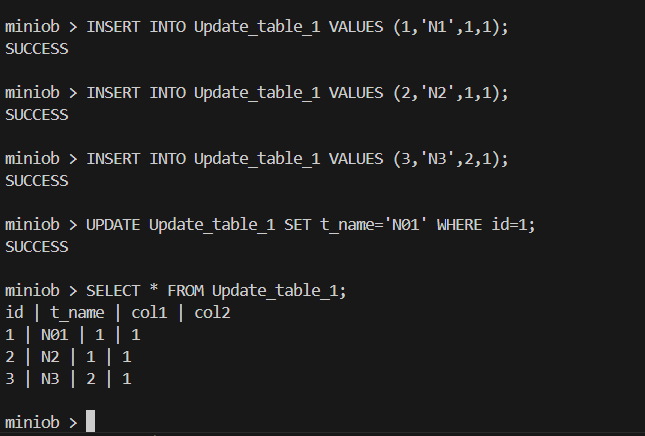
\includegraphics[width=0.3\textwidth]{update_test.png}
    \item \textbf{JOIN测试}：\\
     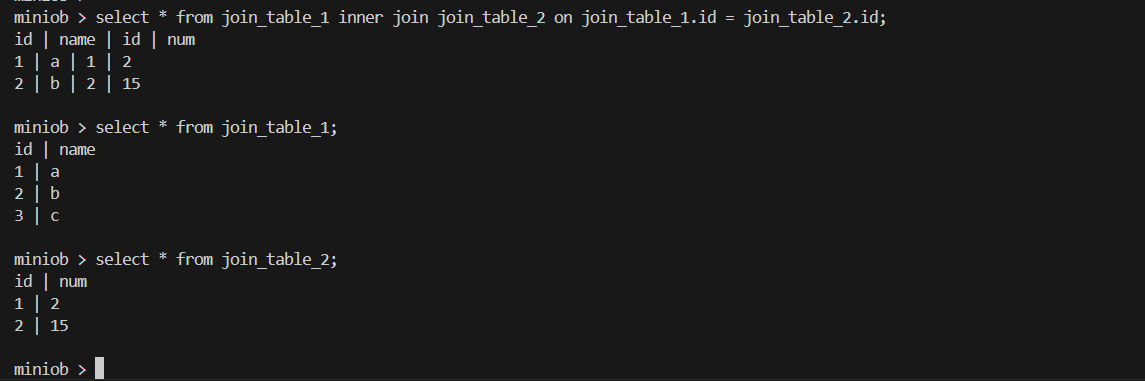
\includegraphics[width=0.3\textwidth]{join_test.png}
     \item \textbf{唯一索引测试-违反唯一约束}：\\
     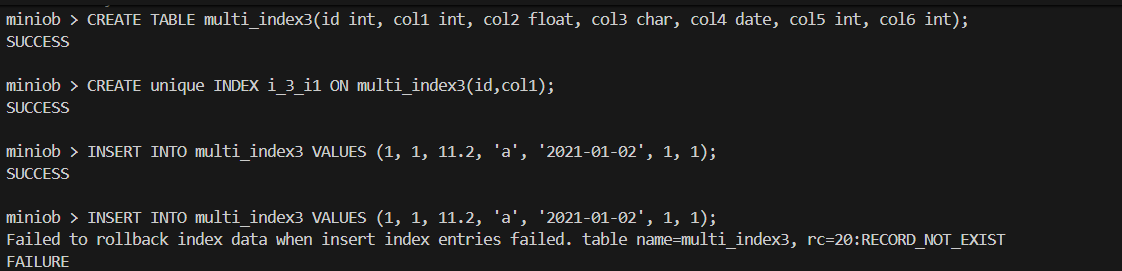
\includegraphics[width=0.3\textwidth]{unique_index_success.png} \\
     \item \textbf{唯一索引测试-唯一约束通过}：\\
    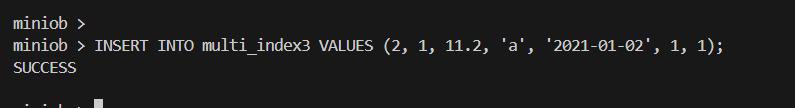
\includegraphics[width=0.3\textwidth]{unique_index_fail.png}
    \item \textbf{子查询测试}：\\
    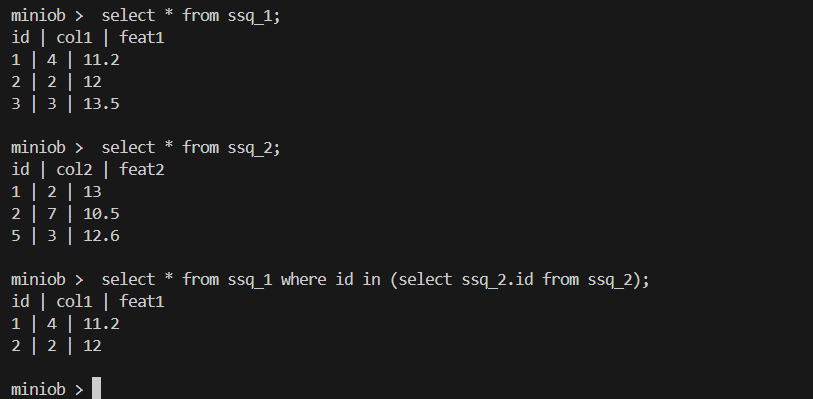
\includegraphics[width=0.3\textwidth]{subquery_test.png}
    \item \textbf{别名测试}：\\
    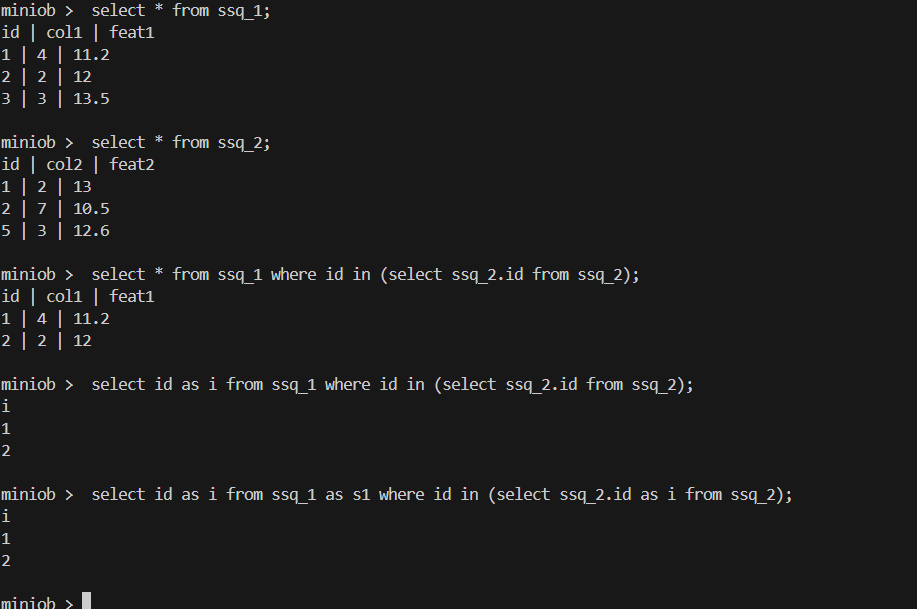
\includegraphics[width=0.3\textwidth]{alias_test.png}
\end{itemize}

\section{总结}
本设计实现了基于MiniOB的数据库核心功能扩展，涵盖：
\begin{itemize}
    \item UPDATE操作的原子性与索引一致性
    \item JOIN查询的优化执行（Hash Join/Nested Loop Join）
    \item 复合索引的前缀扫描与唯一约束
    \item 子查询的标量执行与相关子查询
    \item 别名的多层解析与遮蔽机制
\end{itemize}

\end{document}